%----------------------------------------
% SECTION: Quantum simulation
%----------------------------------------
\section{Quantum simulation}
\label{sec:quantum_simulation}

Simulating quantum mechanics is a very challenging task \cite{manin1980computable, feynman1982simulation}, especially if one is interested in many-body systems.
The description of a state requires a large number of variables, for keeping track of all the quantum amplitudes, and it grows exponentially with the system size.
Hence, one would have an \emph{exponential explosion} in terms of \emph{classical} resources (like for example computer memory), which clearly is not suitable.

If simulating a quantum system is not a task for classical machines, then it should be a task for quantum machines \cite{feynman1982simulation, georgescu2014simulation, hauke2012simulators, kendon2010quantum, buluta2009simulators}.
The possibility of using quantum devices for simulating physics was first envisioned by Feynman in his seminal talk \cite{feynman1982simulation}.
The main idea is to encode the \ac{dof} of an ideal mathematical model of a physically relevant system into a controllable and reliable quantum system.
In other words, a \emph{quantum simulator} is an experimental system that mimics a simple model, or a family of simple models \cite{hauke2012simulators}.
Using quantum physics for simulating quantum physics itself may seem like fighting fire with fire, but it is actually a powerful idea.
We will no longer need an exponentially large number of variables for describing the target system, because the \ac{dof} of the target system and the simulator would be in a one-to-one correspondence.
Therefore, the size of a quantum computer would only be proportional to the size of the quantum system it intends to simulate, \emph{without} an exponential explosion in \emph{quantum} resources.

In this perspective, it would seem that one would need a specific quantum simulator for simulating a specific class of models.
This is not necessarily true with a \emph{quantum computer} \cite{feynman1985quantum, nielsen2010quantum, schleich2007elements, stolze2008quantum}.
The idea for such a device was put forward in \cite{feynman1982simulation, feynman1985quantum} and it would act as a \emph{universal quantum simulator}.
This has proven by LLoyd in \cite{lloyd1996simulator}.
The caveat is that the target system and its evolution would need some \emph{digitalization} scheme beforehand, because a quantum computer uses discrete \ac{dof}, the \emph{qubits}, so they are not suited for continuous-variable computation.
This is analogous to the case of classical computers, where real numbers have to be truncated and represented with a finite-size register of bits.
On the other hand, a problem-specific simulator can potentially uses some kind of physical platform which allows for continuous \ac{dof} \cite{kendon2010quantum, wagner2010continuous}.
% What he put forward was the idea of a new kind of device, the \emph{quantum computer}, which would act as a \emph{universal quantum simulator}.
% This kind of devices, first envisioned from Feynman \cite{feynman1982simulation}, promises much more than simulating quantum mechanics.
% From the works \cite{manin1980computable, feynman1982simulation}, much more than quantum simulation was born and, to this day, quantum computation and quantum information are still very active research fields \cite{feynman1985quantum, nielsen2010quantum, schleich2007elements, stolze2008quantum}.

% A quantum computer can encode the large number of variables of a quantum system in its wave-function.
% In fact, a quantum computer can indeed be used as a \emph{universal quantum simulator} and this fact has been proven by \citeauthor{lloyd1996simulator} in \cite{lloyd1996simulator}.
% Using quantum computers as quantum simulators is basically the idea behind \emph{Digital \acl{qs}}.

% There is another kind of approach to quantum simulation, where one can mimic the evolution of a given quantum system by means of another \emph{analogous} and \emph{controllable} quantum system.
% Hence, we will only need a specific quantum machine for a specific class of problems and a full general-purpose quantum computer is not needed.
% % In this case, for a specific set of problems the full implementation of a quantum computer may not be necessary.
% This is the idea behind \emph{analog \acl{qs}}.

In general, \emph{\acf{qs}} can be (loosely) defined as simulating a quantum system by quantum mechanical means.
There are three paths that can be taken in this regard \cite{georgescu2014simulation}:
\begin{itemize}
    \item Digital \acl{qs}
    \item Analog \acl{qs}
    \item Quantum Information inspired algorithms for classical simulation
\end{itemize}
We will discuss briefly each one of them.
By \emph{quantum simulator} we mean a \emph{controllable} quantum system used to simulate or emulate other quantum systems.
We see that only digital and analog \ac{qs}s employ a quantum simulator.
The last option employs techniques, inspired by quantum information theory, that make it possible to truncate and approximates quantum states in order to have efficient classical simulations.


\begin{figure}[t]
    \centering
    \begin{tikzpicture}[
    ket/.style = {font=\Large},
    ->/.style={-stealth, ultra thick, shorten >=3pt, shorten <=3pt, Grey60},
    system/.style = {draw, dotted, thick, rounded corners, inner sep=10pt},
    simulator/.style = {draw, thick, rounded corners, inner sep=10pt}
    ]
    \node[ket] (phi0) at (0, 2.5) {$\ket{\phi(0)}$};
    \node[ket] (phit) at (3, 2.5) {$\ket{\phi(t)}$};
    \node[ket] (psi0) at (0, 0) {$\ket{\psi(0)}$};
    \node[ket] (psit) at (3, 0) {$\ket{\psi(t)}$};

    \begin{scope}[on background layer]
        \node[fit=(phi0) (phit), system, label=above:{Quantum System}, fill=Blue, fill opacity=0.1] {};
        \node[fit=(psi0) (psit), simulator, label=above:{Simulator}, fill=Blue, fill opacity=0.1] {};
    \end{scope}

    \path (phi0) edge[->] node[above, black] {$U$} (phit);
    \path (psi0) edge[->] node[above, black] {$U^{\prime}$} (psit);

    \path (phi0) edge[->, dashed] (psi0);
    \path (psit) edge[->, dashed] (phit);

    \node (prep) at (0, -1.5) {preparation};
    \node (meas) at (3, -1.5) {measurement};

    \path (prep) edge[->] (psi0);
    \path (psit) edge[->] (meas);
\end{tikzpicture}

    \caption{Schematic picture of a quantum simulator.}
\end{figure}



\subsection{Digital quantum simulations}
\label{sub:digital_quantum_simulations}

The digital approach to \ac{qs} employs the \emph{circuit model} of quantum computation \cite{nielsen2010quantum, deutsch1989quantum}.
This model is analogous to the circuit model of classical computation, where one works with \emph{bits}, the smallest possible amount of information, an on--\emph{or}--off state, and a minimal set of \emph{logical operators} (like \texttt{NOT}, \texttt{AND}, \texttt{OR}, etc\dots).
In quantum computation, the set up is the same but with some key differences:
bits are substituted with \emph{qubits} and the logical operators with \emph{unitary operators}.

A bit can only have two values, either $0$ or $1$.
In quantum computing these values are elevated to two \emph{orthonormal} states $\ket{0}$ and $\ket{1}$.
Therefore, the bits are substituted with \emph{qubits}, which are two-levels quantum systems.
A generic state of a qubit is $\ket{\psi} = \alpha \ket{0} + \beta \ket{1}$, with the normalization condition $\alpha^2 + \beta^2 = 1$, and the complex amplitudes $\alpha$ and $\beta$ encodes the carried information.
A visual representation of the Hilbert space of a qubit is given by the Bloch sphere \todo{inserire figura}.
A set of qubits is called a \emph{quantum register} and they encode the state of the quantum computational machine, the equivalent of the tape of a Turing machine.

The logical operators, or \emph{gates}, of classical computation are single-bit or double-bit functions that have only a single-bit output.
This makes classical computation \emph{non-reversible}\footnote{%
    There exist models of classical computation that are reversible, see \cite{fredkin1982logic}, which will not be discussed here and are not very common in every-day applications.
    In \cite{fredkin1982logic} a universal \emph{three-bits} gate is introduced that allows for reversible computation.%
}.
The idea behind quantum computing is to use the time-evolution of an ad-hoc quantum machine for performing computation.
Time-evolution is a \emph{unitary} process, which means that is reversible.
Hence, the non-reversible model of classical computation is not suited for quantum computing.
There is no one-to-one correspondence between the operations on a classical machine and those on a quantum machine.
Logical operations on a quantum computer, also called \emph{quantum gates}, have to implemented through \emph{unitary operators} that act on the quantum register.
A succession of logical operator, therefore, is equivalent to the product of these unitary operators.
This makes the whole computation a unitary process, hence reversible.

It is known, in classical computing, that only a minimal set of logical gates are actually needed in order to perform any computation.
For example, with a \texttt{NOT} gate and a \texttt{AND} gate is possible to implement every other possible logical function (actually only the \texttt{NAND} gate is necessary).
A similar result is true also for quantum computing \cite{barenco1995gates}.
One only needs a minimal set of quantum gates in order to implement any unitary operators with arbitrary precision.
Similar to the classical case, for quantum computing we only need single-qubit and two-qubits gates.
The two-qubits gates have an important role, because they allow to introduce \emph{entanglement}, which is the secret ingredient that makes quantum computing distinct from classical computing.
This minimal set usually entails a set of single-qubit and one two-qubits entangling gate (like the \texttt{CNOT} gate).
\todo{inserire qualche figura}

\medskip

Even though it has been proven that ``anything'' can be simulated on a quantum computer \cite{lloyd1996simulator}, not all unitary operations can be simulated \emph{efficiently}.
The time-evolution of the target quantum system requires \emph{digitalization}, which means that it has to be decomposed in smaller steps in order to be encodable as a sequence of quantum gates.
This is possible to an arbitrary precision thanks to the Trotter-Suzuki product formula for the exponentiation of complex matrices:
\begin{equation}
    e^{A + B}  = \lim_{n \to \infty} \qty( e^{A/n} e^{B/n} )^n.
\end{equation}
In most physically interesting case, the Hamiltonian is a sum of non-commuting terms:
\begin{equation*}
    H = \sum_{l} H_{l},
\end{equation*}
where $\comm{H_l}{H_{l^{\prime}}} \neq 0$ for $l \neq l^{\prime}$.
In the case of a time-independent Hamiltonian, the time-evolution operator is given by
\begin{equation}
    U(t) = e^{-i t \sum_{l} H_l }
    \quad \text{such that} \quad
    U(t) \ket{\psi(0)} = \ket{\psi(t)}.
    \label{eq:time_evolution_operator}
\end{equation}
In order to implement \eqref{eq:time_evolution_operator} on a quantum operator, the time-evolution has to be divided in $N$ steps of length $\Delta t$, such that $t = N \Delta t$ and $U(t) \simeq (U(\Delta t))^N$.
For each single time step we can apply the first-order Trotter-Suzuki formula \cite{nielsen2010quantum, somma2002simulating} for the time-evolution operator:
\begin{equation}
    U(\Delta t)
    = e^{- i \Delta t \sum_{l} H_l}
    = \prod_{l} e^{-i \Delta t H_l} + O(\Delta t^2).
    \label{eq:trotter_time_evolution}
\end{equation}

The drawback of Trotterization is that high accuracy comes at the cost of very small $\Delta t$ and therefore a very large number of quantum gates.
The scheme used in \eqref{eq:trotter_time_evolution} has some shortcomings, that can be improved with higher order decompositions that will necessarily introduce more complexities in the quantum circuit.
Moreover, some other types of methods have to be used in the case of time-dependent Hamiltonians \cite{wiebe2011simulation}.

\medskip

It should be stressed that we are still far from perfect digital quantum computation.
A typical quantum computer is affected by noise due to its interaction with the environment.
The effect of noise can corrupt the state of the quantum register, by flipping or dephasing the qubits for example.
Furthermore, interaction with an external environment will necessarily lead to \emph{decoherence} where all the ``quantumness'' of the system is lost \cite{zurek1991decoherence, schlosshauer2014decoherence, schlosshauer2019decoherence}.

It becomes clear that error correction is a necessity for \emph{fault-tolerant quantum computing} \cite{preskill1997faulttolerant, shor1996faulttolerant} but it can greatly increase the number of qubits needed for useful computations.
Indeed, it is said we are currently living in the \emph{noisy intermidiate-scale quantum} (NISQ) era of quantum computing \cite{preskill2018quantumcomputing}.
The term refers to moderately sized quantum computers (around 50--100 qubits) whose gates are still affected by noise but are not large enough to fully implement error correction.

\medskip

The typical setup for a digital simulation consists of three steps:
\begin{description}
    \item[Initial-state preparation] the quantum register is prepared in the initial state $\ket{\psi(0)}$.
        This step can be difficult by itself, and it is not always guaranteed that an efficient algorithm may exist.

    \item[Unitary evolution]  the circuit has to reproduce or simulate the action of a unitary operator $U$.
        This unitary operator is usually the time-evolution operator of the target system, which has to be decomposed in a sequence of smaller operation through trotterization, as explained before.

    \item[Final measurement] after obtaining the wanted state $\ket{\psi(t)} = U \ket{\psi(0)}$, a \emph{measurement} is needed in order to extract relevant physical information.
        Instead of capturing the whole wave function $\ket{\psi(t)}$, with, for example, quantum tomography, one may proceed with the direct estimation of certain physical quantities, such as correlation functions or spectra of operators.
\end{description}


\todo{cosa altro aggiungere?}

\begin{figure}[t]
    \centering
    \newcommand{\Gate}[3]{\draw[gate] (#1, -#2 + 0.25) rectangle ++(1.5, -#3 - 0.5);}
    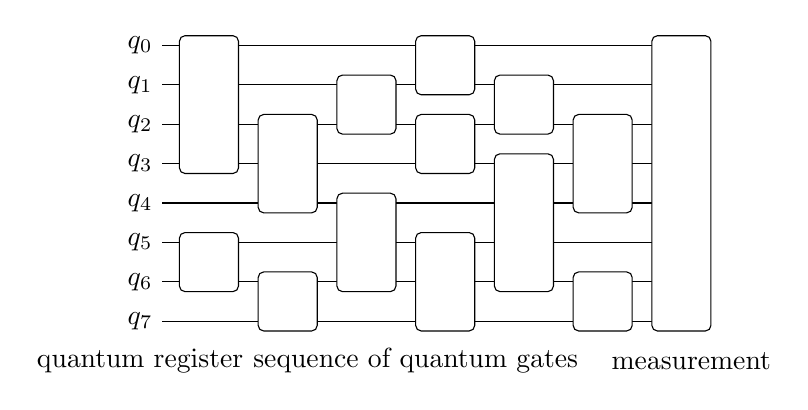
\begin{tikzpicture}[
        scale=0.5,
        gate/.style = {rounded corners=2pt, fill=white}
        ]
        \foreach \n in {0,...,7} {
            \node (q\n) at (0, -\n) {$q_{\n}$};
            \node (q\n end) at (14, -\n) {};
            \path (q\n) edge (q\n end);
        }
        % \draw[gate] (1, 0 + 0.25) rectangle ++(1.5, -3 - 0.5);
        \Gate{1}{0}{3}
        \Gate{1}{5}{1}
        \Gate{3}{2}{2}
        \Gate{3}{6}{1}
        \Gate{5}{1}{1}
        \Gate{5}{4}{2}
        \Gate{7}{5}{2}
        \Gate{7}{2}{1}
        \Gate{7}{0}{1}
        \Gate{9}{3}{3}
        \Gate{9}{1}{1}
        \Gate{11}{2}{2}
        \Gate{11}{6}{1}
        \Gate{13}{0}{7}

        \node at (0, -8) {quantum register};
        \node at (7, -8) {sequence of quantum gates};
        \node at (14, -8) {measurement};
    \end{tikzpicture}
    \caption{Example of a quantum circuit \todo{da finire}.}
\end{figure}


\subsection{Analog quantum simulations}
\label{sub:analog_quantum_simulations}

Analog \ac{qs} (AQS) represent another kind of approach to \ac{qs}, where a one quantum system mimics or emulate another.
The Hamiltonian of the system to be simulated, $H_{\text{sys}}$, is directly mapped onto the Hamiltonian of the quantum simulator, $H_{\text{sim}}$.
Obviously, this can be done if there is a mapping between the system and the simulator.
Note that the simulator may only partly reproduce the dynamics of the system, or simulate some effective description of the system.

An important advantage of analog \ac{qs} is that it does not require a full quantum computer.
Even more, the simulator does not even need to be a computer at all.
Finding the mapping in an analog \ac{qs} might look, at first, simpler than finding the most efficient gate decomposition of a Hamiltonian, but it is not always true and there are no recipes ready for constructing these mappings in a general case.
The obvious drawback of AQS is that the quantum simulators are problem specific, but on the other hand, given that they do not require a full quantum computer, they are more feasible in the near-term.


\todo{Aggiungere altro ma cosa?}


\subsection{Quantum-inspired algorithms}
\label{sub:quantum_inspired_algorithms}

Thanks to the developing science of quantum information, new \emph{classical algorithms} have been invented for the simulation of quantum many-body systems.
One of the most important examples of these quantum-inspired algorithms are \emph{tensor networks} methods\todo{inserire citazioni di review}\citneeded.

Tensor networks make it possible to ``compress'' the information about a many-body wave function by expressing it as a contraction of a network of tensors (as suggested by the name).
In details, to each physical site we associate a tensor with a number of indices (or legs).
One of these indices is called the \emph{physical index} of the tensors, which runs over the basis of the local Hilbert space.
The other indices are \emph{auxiliary indices}, their dimension is governed by a parameter $\chi$ called the \emph{bond dimension} and are ``connected'' to other sites.
Roughly speaking, these auxiliary indices encodes the entanglement information between the connected sites.

For a large class of physically relevant models, the ground state is gapped and has, in a certain sense, a finite amount of entanglement.
This fact is expressed by the so-called \emph{area law}, where the entanglement between two partitions of the system grows with size of the boundary, the area between the two partitions, and not with the size of the partition itself.
The main advantage of tensor networks is their ability to capture this area law.

\todo{Aggiungere altro}
